\section{Superfici di Controllo}
Le superfici di controllo sono dei dispositivi in grado di modificare l'assetto del velivolo. Sono controllate dal pilota o dall'autopilota.

\begin{itemize}
    \item \textbf{Alettoni}: sono posizionate all'estremità delle ali. Operano in modalità differenziale: quando uno si alza, l'altro si abbassa.
          Il loro movimento influenza l'angolo di rollio $\phi$ dell'aeromobile.
          Sono controllati ruotando la cloche e la loro deflessione è indicata con $\delta_a (t)$;
    \item \textbf{Equilibratore}: è la parte mobile del piano orizzontale di coda di un aeromobile. I due lati si muovono all'unisono.
          Il suo movimento influenza l'angolo di beccheggio $\theta$ dell'aeromobile.
          È controllato mediante la traslazione avanti e indietro della cloche e la sua deflessione è indicata con $\delta_e (t)$;

    \item \textbf{Timone}: è una superficie di controllo montata al piano verticale di coda.
          Il suo movimento influenza l'angolo di imbardata $\psi$ dell'aeromobile.
          È controllato attraverso i pedali e la sua deflessione è indicata con $\delta_r (t)$;
\end{itemize}

\begin{figure}[H]
    \centering
    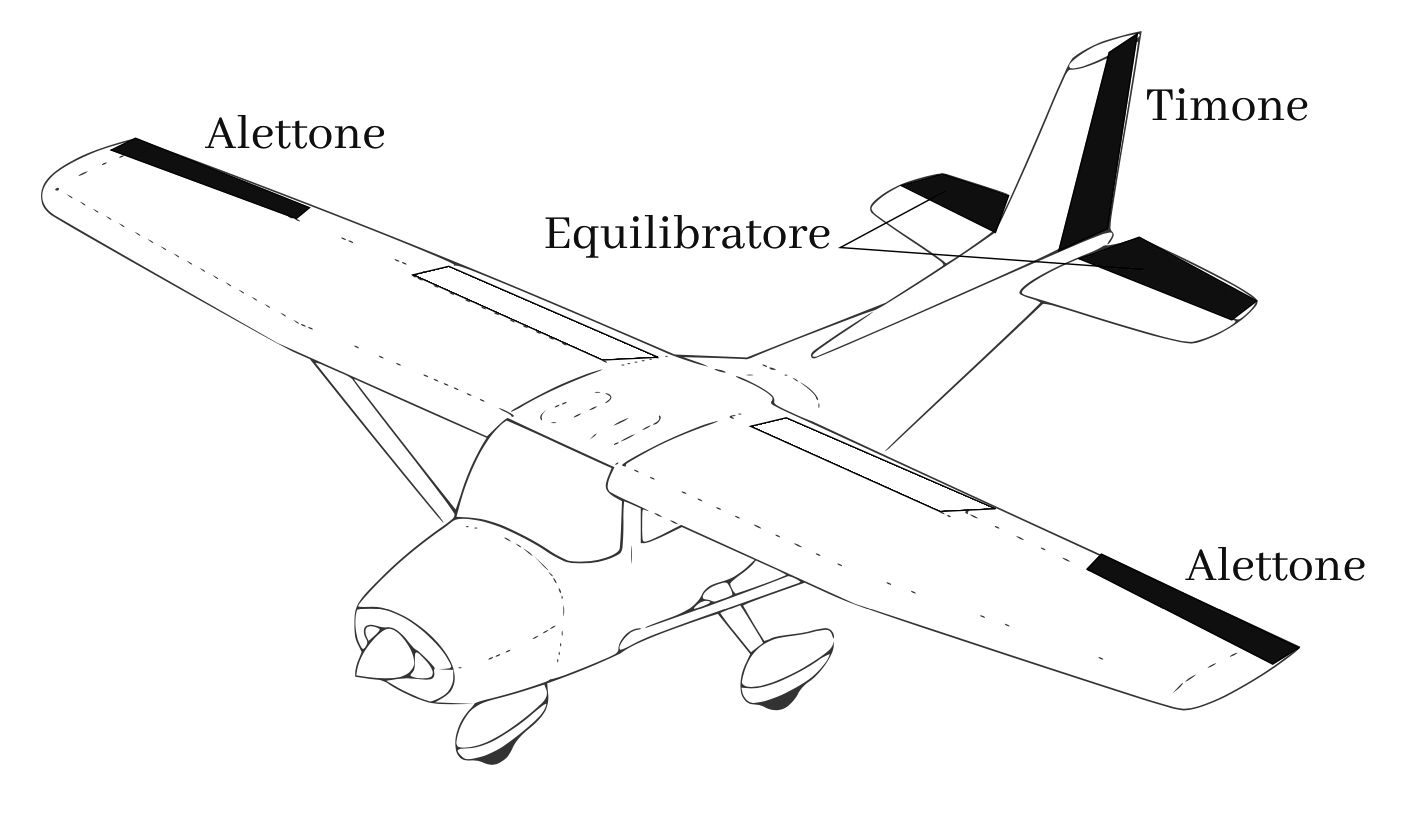
\includegraphics[width=0.55\linewidth]{Immagini/ControlSurfaces.jpg}
    \caption{Superfici di Controllo \cite{smith_aircraft_flight_mechanics}}
\end{figure}
